\documentclass[border=3pt]{standalone}
\usepackage{tikz}
\usetikzlibrary{arrows.meta,calc}
\tikzset{pin/.style={-{Stealth[length=5pt]}}}
\begin{document}
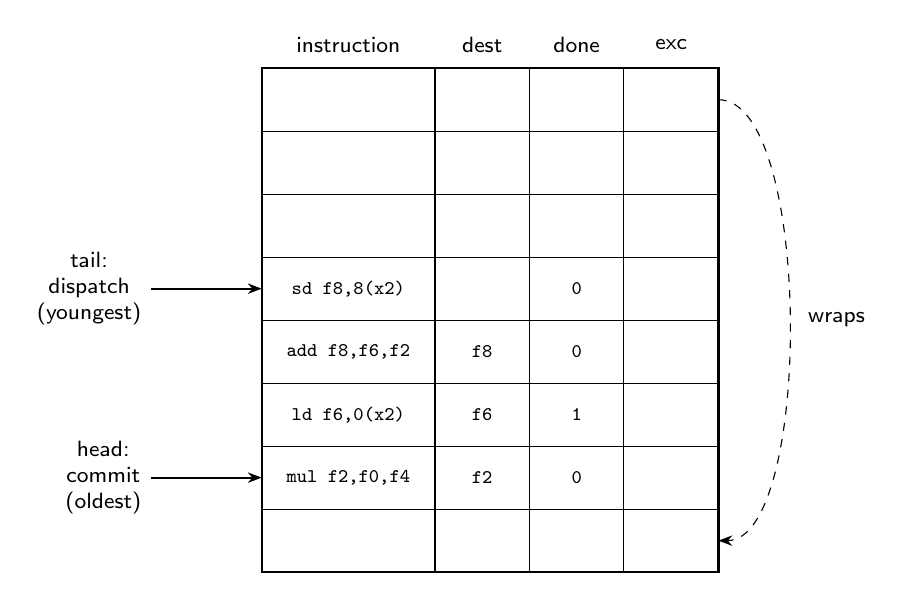
\begin{tikzpicture}[font=\sffamily\small, x=1mm, y=1mm]
  % ROB as a vertical array, entries 0..7
  \draw[thick] (0,0) rectangle (58,64);
  \foreach \y in {8,16,24,32,40,48,56}{\draw (0,\y) -- (58,\y);}
  % columns: instr | dest | value | done | exc
  \foreach \x in {22,34,46}{\draw (\x,0) -- (\x,64);}
  \node[font=\sffamily\footnotesize] at (11,67) {instruction};
  \node[font=\sffamily\footnotesize] at (28,67) {dest};
  \node[font=\sffamily\footnotesize] at (40,67) {done};
  \node[font=\sffamily\footnotesize] at (52,67) {exc};
  % some contents (oldest at bottom)
  \node[font=\ttfamily\scriptsize] at (11,12) {mul f2,f0,f4};
  \node[font=\ttfamily\scriptsize] at (28,12) {f2};  \node[font=\ttfamily\scriptsize] at (40,12) {0};
  \node[font=\ttfamily\scriptsize] at (11,20) {ld f6,0(x2)};
  \node[font=\ttfamily\scriptsize] at (28,20) {f6};  \node[font=\ttfamily\scriptsize] at (40,20) {1};
  \node[font=\ttfamily\scriptsize] at (11,28) {add f8,f6,f2};
  \node[font=\ttfamily\scriptsize] at (28,28) {f8};  \node[font=\ttfamily\scriptsize] at (40,28) {0};
  \node[font=\ttfamily\scriptsize] at (11,36) {sd f8,8(x2)};
  \node[font=\ttfamily\scriptsize] at (40,36) {0};
  % head / tail pointers
  \draw[pin, thick] (-14,12) node[left, align=center, font=\sffamily\footnotesize]{head:\\commit\\(oldest)} -- (0,12);
  \draw[pin, thick] (-14,36) node[left, align=center, font=\sffamily\footnotesize]{tail:\\dispatch\\(youngest)} -- (0,36);
  % wrap arrow
  \draw[pin, dashed] (58,60) .. controls (70,60) and (70,4) .. (58,4);
  \node[font=\sffamily\footnotesize, rotate=0] at (73,32) {wraps};
\end{tikzpicture}
\end{document}
